% #####################################################################
% #####################################################################
% ##                                                                 ##
% ##                             Lizenz:                             ##
% ##                         CC BY-NC-SA 3.0                         ##
% ##      http://creativecommons.org/licenses/by-nc-sa/3.0/de/       ##
% ##                                                                 ##
% #####################################################################
% ##   Diese Datei kann beliebig verändert werden, solange darauf    ##
% ##     hingewiesen wird, dass dieses Dokument ursprünglich von     ##
% ##                                                                 ##
% ##                        www.ei-studium.de                        ##
% ##                                                                 ##
% ##                             stammt.                             ##
% ## Dies gilt insbesondere auch für alle daraus erstellten Dateien. ##
% ##    Des Weiteren muss die Weitergabe dieser Dateien unter der    ##
% ##                    gleichen Lizenz erfolgen.                    ##
% #####################################################################
% #####################################################################
\documentclass[a4paper,twocolumn,10pt]{article}
\usepackage[utf8]{inputenc}
\usepackage[ngerman]{babel}
\usepackage[top=2.0cm,bottom=1.5cm,left=1.0cm,right=1.0cm]{geometry}
\usepackage{enumitem}
\usepackage{graphicx}
\usepackage{amsfonts}
\usepackage{amsmath}
\usepackage{sectsty}
\usepackage{colortbl}
\usepackage{cancel}
\usepackage{listings}
\usepackage{color}
\usepackage{amsmath}
\usepackage{trfsigns}
\usepackage{epstopdf}
\usepackage{amssymb}
\usepackage{fancyhdr}
\usepackage[pdfborder={0 0 0}]{hyperref}

\setlist{itemsep=.01mm}
\setenumerate{label=\emph{\arabic*})}
\setlength{\columnsep}{1cm}
\parindent 0mm

\partfont{\Large}
\sectionfont{\large \sc\bf}
\subsectionfont{\normalsize}
\subsubsectionfont{\small\textit}

\pagestyle{fancy}
\lhead[\leftmark]{Formelsammlung Mathematik 4 für EI}
\chead[\leftmark]{\url{http://www.ei-studium.de}}
\rhead[\leftmark]{Erstelldatum: \today}
\lfoot[\leftmark]{Keine Garantie auf Vollständigkeit und Richtigkeit!}
\cfoot[\leftmark]{}
\rfoot[\leftmark]{\thepage}
\renewcommand{\headrulewidth}{0.5pt}
\renewcommand{\footrulewidth}{0.5pt}

\begin{document}
\tableofcontents
\newpage

\part{Mathematik 4}

\section{Wiederholung}

\subsection{Matrixnormen}
Sei $||.||$ eine Norm auf $\mathbb{R}^n,n\geq 1$, dann definiert
\begin{equation*}
|||A|||=\sup\limits_{x\neq 0}\frac{||Ax||}{||x||}=\max\limits_{||x||=1}||Ax||
\end{equation*}
für $A\in\mathbb{R}^{n\times n}$ eine Norm.\\
Außerdem gilt:
\begin{enumerate}
\item Submultiplikativität
\begin{equation*}
|||AB|||\leq |||A|||\cdot |||B|||
\end{equation*}
\item Verträglichkeit
\begin{equation*}
||Ax||\leq |||A|||\cdot ||x||
\end{equation*}
\end{enumerate}
Die von der \textbf{Maximumsnorm} $||.||_{\infty}$ induzierte Matrizennorm ist die ''maximale Zeilensumme''.
\begin{equation*}
||A||_{\infty}=\max\limits_{1\leq i\leq n}\sum\limits_{j=1}^{n}|a_{ij}|
\end{equation*}
Die von der \textbf{$l_1$-Norm} $||.||_1$ induzierte Matrizennorm ist die ''maximale Spaltensumme'':
\begin{equation*}
||A||_1=\max\limits_{1\leq j\leq n}\sum\limits_{i=1}^{n}|a_{ij}|
\end{equation*}
Sei $A$ eine symmetrische Matrix, dann gilt:
\begin{equation*}
||A||_2 =|\lambda_{max}|=\{|\lambda|\;|\lambda\in\mathbb{R}\;ist\;Eigenwert\;von\;A\}
\end{equation*}
Für beliebige $\mathbb{R}^{n\times n}$-Matrizen gilt:
\begin{equation*}
||A||_2=\sqrt{\lambda_{\text{max}}(A^TA)}=\rho (A^TA)^{\frac{1}{2}}\;\;\;\;\;(\text{Spektralradius})
\end{equation*}
Die Eigenwerte von $A$ und $A^{-1}$ sind zueinander invers.
\begin{equation*}
\Rightarrow||A^{-1}||_2=\frac{1}{\sqrt{\lambda_{\text{min}}(A^TA)}}
\end{equation*}

\subsection{Wichtige Reihen}
\begin{equation*}
\begin{split}
\ln(1+x)&=\sum\limits_{k=0}^{\infty}\frac{(-1)^k}{k+1}x^{k+1}=x-\frac{x^2}{2}+\frac{x^3}{3}-...,\;x\in (-1,1]\\
\sin(x)&=\sum\limits_{k=0}^{\infty}(-1)^k\frac{x^{2k+1}}{(2k+1)!}=x-\frac{x^3}{3!}+\frac{x^5}{5!}-...\\
\cos(x)&=\sum\limits_{k=0}^{\infty}(-1)^k\frac{x^{2k}}{(2k)!}=1-\frac{x^2}{2!}+\frac{x^4}{4!}-...\\
e^x&=\sum_{k=0}^{\infty}\frac{x^k}{k!}=1+x+\frac{x^2}{2!}+\frac{x^3}{3!}+...
\end{split}
\end{equation*}
Für alternierende Reihen $\sum_{k=0}^{\infty}(-1)^ka_k$ mit $a_k\leq 0$ und monoton fallend (z.B. $\ln,\sin,\cos$) gilt nach dem \textbf{Leibnizkriterium}:
\begin{equation*}
\underbrace{\left|\sum_{k=0}^{\infty}(-1)^ka_k-\sum_{k_0}^{N}(-1)^ka_k\right|}_{\text{Restglied}}\leq a_{N+1}
\end{equation*}
Für die Exponentialreihe gilt:
\begin{equation*}
\underbrace{\left|e^x-\sum_{k=0}^{N}\frac{x^k}{k!}\right|}_{\text{Restglied}}\leq 2\cdot\frac{|x^{N+1}|}{(N+1)!}\;\;\;\text{für}\; |x|\leq 1
\end{equation*}

\section{Grundbegriffe der Numerik}

\subsection{Gleitkomma-Arithmetik}
Es werden Zahlen der Form
\begin{equation*}
a=(-1)^s\cdot m\cdot b^e
\end{equation*}
betrachtet, mit $b\in\mathbb{N}, b\geq 2,\;s\in\{0,1\}$ und
\begin{equation*}
\begin{split}
m&=\sum_{i=0}^{t-1}m_ib^{-i};\;\;\;\;m_i\in\{0,...,b-1\}\\
e&=\sum_{i=0}^{r-1}e_ib^i-\underbrace{(b^{r-1}-1)}_{\text{bias}}; \;\;\;\;e_i\in\{0,...,b-1\}
\end{split}
\end{equation*}
wobei $t\geq 2$ und $r\geq 2$ die Genauigkeiten darstellen.\\\\
Nachfolgend sei $b=2$.\\\\
IEEE ''single'':\\
32 Bit ($s$: 1 Bit, $e$: 8 Bit, $m$: 23 Bit)\\
IEEE ''double'':\\
64 Bit ($s$: 1 Bit, $e$: 11 Bit, $m$: 52 Bit)\\\\
\underline{Definitionen:}
\begin{enumerate}[label=$\bullet$]
\item $a\in\mathbb{R}$ heißt \textbf{normierte Gleitkommazahl} ($a\in\mathbb{M}_{t,r}^N$), falls eine Darstellung existiert mit $m_0=1$ und $e_{\text{min}}<e<e_{\text{max}}$, wobei gelte:
\begin{equation*}
\begin{split}
e_{\text{min}}&=-b^{r-1}+1\\
e_{\text{max}}&=b^{r-1}
\end{split}
\end{equation*}
\item $a\in\mathbb{R}$ heißt \textbf{subnormale Gleitkommazahl} ($a\in\mathbb{M}_{t,r}^S$), falls $e=e_{\text{min}}$ und $m_0=0$, wobei nicht alle $m_i$ Null sind.
\begin{equation*}
\Rightarrow a=(-1)^s\left(\sum_{i=1}^{t-1}m_i2^{-i}\right)2^{e_{\text{min}}+1}
\end{equation*}
\item Sonderfälle
\begin{enumerate}[label=-]
\item ''0'': $\forall i: m_i=0,e_i=0$
\item ''$\infty$'': $\forall i: m_i=0, e_i=1$
\item ''NaN'': $\forall i: e_i=1$, wobei nicht alle $m_i$ Null sind.
\end{enumerate}
\item $\mathbb{M}_{t,r}=\mathbb{M}_{t,r}^N\cup\mathbb{M}_{t,r}^S\cup\{\pm\infty\}\cup\{NaN\}$
\item Der Abstand von $1$ zur nächstgrößeren Zahl in $\mathbb{M}_{t,r}$ ist:
\begin{equation*}
\text{eps}=2^{-(t-1)}\;\;\;\;\text{(Maschinengenauigkeit)}
\end{equation*}
\item Rundung: $\text{rd}_{t,r}:\mathbb{R}\rightarrow\mathbb{M}_{t,r}^N$
\end{enumerate}
Für die IEEE-754-Standardrundung gilt:
\begin{equation*}
\frac{|x-\text{rd}_{t,r}|}{|x|}\leq\frac{\text{eps}_t}{2}\;\text{für}\;x\neq 0
\end{equation*}
Für alle $x,y\in\mathbb{M}_{t,r}^N$ und $*\in\{+,-,\cdot,/\}$ gilt:
\begin{equation*}
x\circledast y=\text{rd}_{t,r}(x*y)
\end{equation*}

\subsection{Kondition}
Seien $x,y$ normierte Vektorräume (mit Norm $||.||$).\\
Ein Problem ist eine Funktion $f:x\rightarrow y$.\\
Gesucht ist $\delta f=f(x+\delta x)-f(x)$ im Vergleich zu $\delta x$.\\\\
Die \textbf{absolute Kondition} von $f$ im Punkt $x\in X$ ist
\begin{equation*}
\kappa_{\text{abs}}^f(x)=\lim\limits_{\delta\rightarrow 0}\sup\limits_{||\delta x||<\delta}\frac{||\delta f||}{||\delta x||}
\end{equation*}
Sei $f:\mathbb{R}\rightarrow\mathbb{R}$ differenzierbar (mit $||.||=|.|$), dann gilt:
\begin{equation*}
\kappa_{\text{abs}}(x)=|f'(x)|
\end{equation*}
\begin{equation*}
\Rightarrow||\delta f||\leq \kappa_{\text{abs}}\cdot ||\delta x||
\end{equation*}
Für die \textbf{relative Kondition} gilt:
\begin{equation*}
\kappa_{\text{rel}}(x)=\lim\limits_{\delta\rightarrow 0}\sup\limits_{||\delta x||<\delta} \frac{\frac{||\delta f||}{||f||}}{\frac{||\delta x||}{||x||}}=\lim\limits_{\delta\rightarrow 0}\sup\limits_{||\delta x||<\delta} \frac{||\delta f||\cdot ||x||}{||f||\cdot ||\delta x||}
\end{equation*}
Sei $f:\mathbb{R}\rightarrow\mathbb{R}$ differenzierbar, dann gilt:
\begin{equation*}
\kappa_{\text{rel}}=\frac{|f'(x)|}{\frac{|f(x)|}{|x|}}=\frac{|f'(x)|\cdot |x|}{|f(x)|}
\end{equation*}
\begin{equation*}
\Rightarrow\frac{||\delta f||}{||f||}\leq \kappa_{\text{rel}}\cdot\frac{||\delta x||}{||x||}
\end{equation*}
Sei $A\in\mathbb{R}^{n\times n},f:\mathbb{R}^n\rightarrow\mathbb{R}^n,b\rightarrow f(b)=A^{-1}b=x$, dann gilt:
\begin{equation*}
\begin{split}
\kappa_{\text{abs}}(b)&=||f'(b)||=||A^{-1}||\\
\kappa_{\text{rel}}(b)&=\frac{||A^{-1}||}{\frac{||A^{-1}b||}{||b||}}=||A^{-1}||\frac{||Ax||}{||x||}\leq||A^{-1}||\cdot ||A||
\end{split}
\end{equation*}
Für die Kondition bzgl. $||.||_2$ gilt außerdem:
\begin{equation*}
\kappa_{\text{rel}}(A)=\sqrt{\frac{\lambda_{\text{max}}(A^TA)}{\lambda_{\text{min}}(A^TA)}}
\end{equation*}
$\mathcal{N.B.}$:
\begin{equation*}
\frac{||f(\tilde{x})-f(x)||}{||f(x)||}\leq \kappa_{\text{rel}}\cdot\frac{||\tilde{x}-x||}{||x||}+O\left(\frac{||\tilde{x}-x||^2}{||x||^2}\right)
\end{equation*}

\subsection{Stabilität}
\underline{Definitionen:}
\begin{enumerate}[label=$\bullet$]
\item Ein \textbf{Algorithmus} ist eine Abb. $\tilde{f}:x\rightarrow y$ mit $\tilde{f}=\tilde{f}_k\circ ...\circ \tilde{f}_1$, wobei jeder Teilschritt $\tilde{f}_i,i=1,...,k$ nur Operationen aus $\{\oplus ,\ominus,\odot,\oslash,\text{rd}\}$ enthält.
\item Ein Algorithmus $\tilde{f}$ für ein Problem $f$ heißt \textbf{rückwärtsstabil}, falls $\forall x\in X\;\exists\;\tilde{x}\in X$ mit
\begin{equation*}
\underbrace{\tilde{f}(x)}_{(1+\epsilon)f(x)}=f(\tilde{x})\;\text{und}\;\frac{||x-\tilde{x}||}{||x||} = O(\epsilon)\text{ für }\epsilon\rightarrow 0
\end{equation*}
wobei $\epsilon$ den relativen Fehler darstellt.
\end{enumerate}
\textbf{Ziel:}\\
Finde zu geg. $f$ ein $\tilde{f}$, sodass der Fehler $||\tilde{f}(x)-f(x)||$ bzw. $\frac{||\tilde{f}(x)-f(x)||}{||f(x)||}$ möglichst ''klein'' ist.\\\\
Sei $\tilde{f}$ ein rückwärtsstabiler Algorithmus für $f$, dann gilt:
\begin{equation*}
\frac{||\tilde{f}(x)-f(x)||}{||f(x)||}\leq O(\kappa_{\text{rel}}(x)\cdot \text{eps})\;\text{für eps}\rightarrow 0
\end{equation*}

\section{Numerische lineare Algebra}

\subsection{Dreiecksmatrizen}
\textbf{Satz:}\\
Falls $A=LR$ mit $L\in\mathbb{R}^{n\times n}$ untere und $R\in\mathbb{R}^{n\times n}$ obere Dreiecksmatrix, $det(A)\neq 0$, so ist das LGS $Ax=b$ für alle $b\in\mathbb{R}^n$ in $2n^2$ Operationen lösbar.\\\\
$\mathcal{N.B.}$
\begin{equation*}
\sum\limits_{k=1}^{n}(ak-b)=\frac{1}{2}n(an+a-2b)
\end{equation*}

\subsubsection{Vorwärts- / Rückwärtssubstitution}
Falls $A$ obere oder untere Dreiecksmatrix, so kann das LGS $Ax=b$ durch Vorwärts- bzw. Rückwärtssubstitution gelöst werden.\\\\
\underline{Matlab-Code für Vorwärtssubstitution:}
\begin{tabbing}
for \= $j=1:n$\\
\>$x(j)=(b(j)-A(j,1:j-1)*x(1:j-1))/A(j,j);$\\
end
\end{tabbing}
\underline{Matlab-Code für Rückwärtssubstitution:}
\begin{tabbing}
for \= $j=n:-1:1$\\
\>$x(j)=(b(j)-A(j,j+1:n)*x(j+1:n))/A(j,j);$\\
end
\end{tabbing}
Aufwand: je $n^2$ Flops

\subsection{Nachiteration}
Mit Hilfe der Nachiteration kann eine Näherungslösung $\tilde{x}$ eines LGS $Ax=b$ genauer approximiert werden.\\\\
\textbf{Vorgehensweise:}
\begin{enumerate}
\item Berechne $\tilde{x}$:
\begin{equation*}
A\tilde{x}=b
\end{equation*}
\item Berechne $r$:
\begin{equation*}
r=b-A\tilde{x}
\end{equation*}
\item Berechne $z$:
\begin{equation*}
Az=r
\end{equation*}
\item Die genauere Näherungslösung $\hat{x}$ lautet:
\begin{equation*}
\hat{x}=\tilde{x}+z
\end{equation*}
\end{enumerate}

\subsection{LR/LU-Zerlegung}
Sei $A\in\mathbb{R}^{n\times n}, det(A)\neq 0,a_{ii}\neq 0, L\in\mathbb{R}^{n\times n}$ untere und $R\in\mathbb{R}^{n\times n}$ obere Dreiecksmatrix.\\
Dann kann das LGS $Ax=b$ wie folgt gelöst werden:
\begin{enumerate}
\item Berechne $L$ und $R$, sodass $A=LR$
\item Berechne $y$, sodass $Ly=b$ (für LRP-Zerlegung: $Ly=Pb$)
\item Berechne $x$, sodass $Rx=y$
\end{enumerate}
Für die Berechnung von $L$ und $R$ wird folgender Algorithmus angewendet:
\begin{enumerate}
\item Setze $l_{i1}=\frac{a_{i1}}{a_{11}}$ für $i\geq 1$.
\item Setze $a_{ij}=a_{ij}-l_{i1}\cdot a_{1j}$ für alle $j$ und $i>1$:
\begin{equation*}
\text{Zeile }i=\text{Zeile }i-l_{i1}\cdot \text{ Zeile }1,\;\;\;\;i>1
\end{equation*}
\item Gehe zu Schritt 1 und ersetze alle 1er durch 2,3,4,...
\end{enumerate}
\vspace{0.3cm}
Beispiel:
\begin{center}
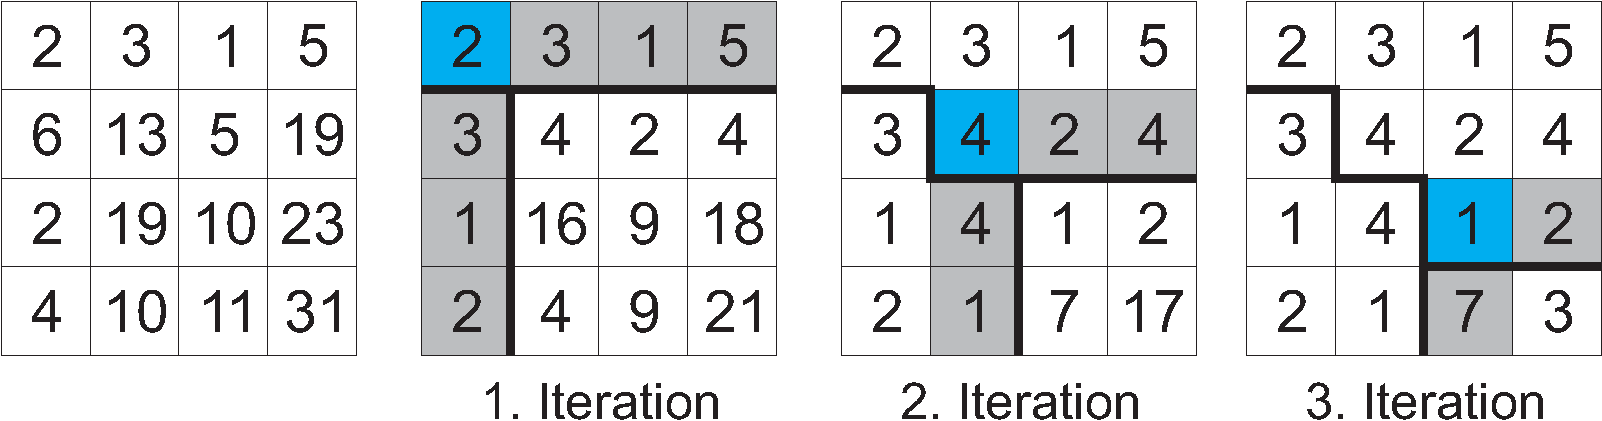
\includegraphics[width=0.95\columnwidth]{Grafiken/LU-Zerlegung}
\end{center}
\begin{equation*}
\Rightarrow\underbrace{\begin{pmatrix}2 & 3 & 1 & 5 \\ 6 & 13 & 5 & 19 \\ 2 & 19 & 10 & 23 \\ 4 & 10 & 11 & 31\end{pmatrix}}_{A}=\underbrace{\begin{pmatrix}1 & 0 & 0 & 0 \\ 3 & 1 & 0 & 0 \\ 1 & 4 & 1 & 0 \\ 2 & 1 & 7 & 1\end{pmatrix}}_{L}\underbrace{\begin{pmatrix}2 & 3 & 1 & 5 \\ 0 & 4 & 2 & 4 \\ 0 & 0 & 1 & 2 \\ 0 & 0 & 0 & 3\end{pmatrix}}_{R}
\end{equation*}
\\Aufwand für Zerlegung: $\frac{2}{3}n^3-\frac{1}{2}n^2-\frac{1}{6}n$ Flops\\\\
Das oben genannte Verfahren ist ein \underline{direktes}/exaktes Lösungsverfahren (keine Verfahrensfehler; nur Rundungsfehler)\\\\
\underline{Matlab-Code:}
\begin{tabbing}
[n,$\sim$] = size(A);\\
for \=k = 1:n\\
    \>I = k+1:n;\\
    \>A(I,k) = A(I,k)/A(k,k);\\
    \>A(I,I) = A(I,I) - A(I,k)*A(k,I);\\
end
\end{tabbing}

\subsection{LRP/LUP-Zerlegung}
Die LRP-Zerlegung ist eine LU-Zerlegung mit Pivoting-Strategie:\\
Suche $j\geq k$, sodass $|a_{jk}^{(k)}|\geq |a_{ik}^{k}|\;\;\forall\; i\geq k$ und vertausche die $j$-te mit der $k$-ten Zeile in $A^{(k)}$.\\\\
Für $det(A)\neq 0$ existiert eine Permutationsmatrix $P\in\mathbb{R}^{n\times n}$, sodass gilt:
\begin{equation*}
PA=LR
\end{equation*}
\textbf{Definition:}\\
Eine Matrix heißt \textbf{Permutationsmatrix}, falls sie in jeder Zeile und jeder Spalte jeweils eine 1 enthält und sonst nur 0.\\\\
Beispiel:
\begin{center}
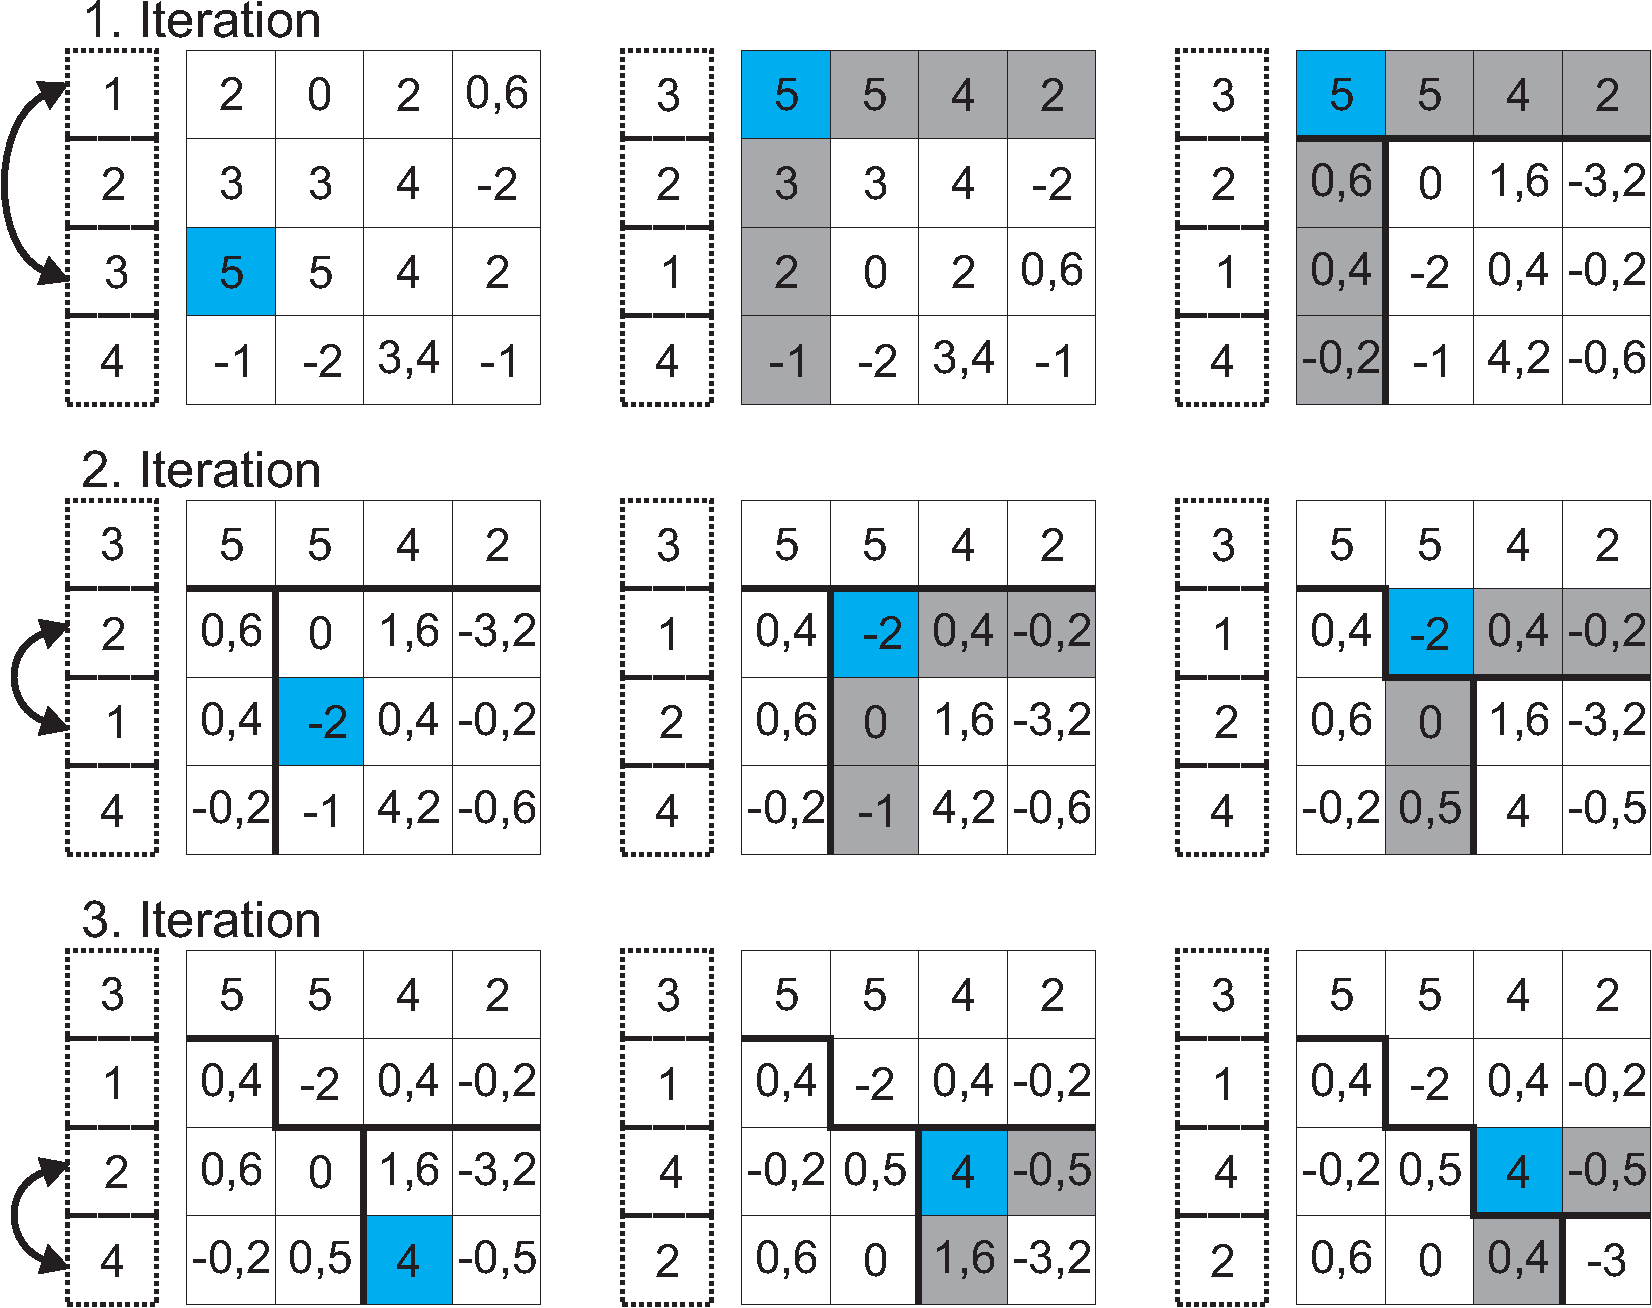
\includegraphics[width=0.95\columnwidth]{Grafiken/LUP-Zerlegung}
\end{center}
\begin{equation*}
\begin{split}
\Rightarrow&\underbrace{\begin{pmatrix}0 & 0 & 1 & 0 \\ 1 & 0 & 0 & 0 \\ 0 & 0 & 0 & 1 \\ 0 & 1 & 0 & 0\end{pmatrix}}_{P}\underbrace{\begin{pmatrix}2 & 0 & 2 & 0,6 \\ 3 & 3 & 4 & -2 \\ 5 & 5 & 4 & 2 \\ -1 & -2 & 3,4 & -1\end{pmatrix}}_{A}\\
&=\underbrace{\begin{pmatrix}1 & 0 & 0 & 0 \\ 0,4 & 1 & 0 & 0 \\ -0,2 & 0,5 & 1 & 0 \\ 0,6 & 0 & 0,4 & 1\end{pmatrix}}_{L}\underbrace{\begin{pmatrix}5 & 5 & 4 & 2 \\ 0 & -2 & 0,4 & -0,2 \\ 0 & 0 & 4 & -0,5 \\ 0 & 0 & 0 & -3\end{pmatrix}}_{R}
\end{split}
\end{equation*}
\underline{Matlab-Code:}
\begin{tabbing}
[n,$\sim$] = size(A);\\
p = 1:n;\\
for \=k = 1:n\\
    \>[$\sim$,j] = max(abs(A(p(k:n),k)));\\
    \>j = j + (k-1);\\
    \>p([k,j]) = p([j,k]);\\
    \>I = k+1:n;\\
    \>A(p(I),k) = A(p(I),k)/A(p(k),k);\\
    \>A(p(I),I) = A(p(I),I) - A(p(I),k)*A(p(k),I);\\
end
\end{tabbing}

\subsection{Cholesky-Zerlegung}
Sei $A\in\mathbb{R}^{n\times n}$ symmetrisch und positiv definit, dann existiert eine rechte obere Dreiecksmatrix $R$ mit
\begin{equation*}
A=R^TR
\end{equation*}
\subsubsection{Rekursiver Algorithmus zur Berechnung von $R$}
\begin{enumerate}
\item Ersetze $a_{11}$ durch $\sqrt{a_{11}}$
\item Ersetze alle Einträge unter $a_{11}$ durch $0$
\item Ersetze alle Einträge rechts von $a_{11}$ durch $\frac{a_{1i}}{a_{11}}$
\item Beende die Funktion, falls $n==1$
\item Um den inneren Teil der Matrix zu berechnen ($A(2:n,2:n)$), rufe die Funktion mit folgender Matrix auf:
\begin{equation*}
A(2:n,2:n)-A(1,2:n)^T\cdot A(1,2:n)
\end{equation*}
\end{enumerate}
Die entstandene Matrix stellt dann $R$ dar.\\\\
Aufwand für Zerlegung: $\frac{1}{3}n^3$ Flops

\subsection{Householder-Spiegelung}
Die Spiegelung $\tilde{x}$ von $x\in\mathbb{R}^k$ an der Hyperebene $E_V$ senkrecht zu $v\in\mathbb{R}^k$ heißt Householder-Spiegelung. Es gilt:
\begin{equation*}
\tilde{x}=\underbrace{\left(I_n-\frac{2vv^T}{||v||^2}\right)}_{H_v\in\mathbb{R}^{m\times m}}\cdot x
\end{equation*}
Sei $v\neq 0$, dann gilt:
\begin{enumerate}[label=$\bullet$]
\item $H_v^T=H_v,H_vH_v=I\Rightarrow H_v$ orthogonal
\item $H_{\alpha v}=H_v\;\forall\;\alpha\in\mathbb{R}\backslash\{0\}$
\item $H_va=\mp ||a||e_1$, falls $v=a\pm ||a||e_1$
\end{enumerate}

\subsection{QR-Zerlegung}
Sei $A\in\mathbb{R}^{m\times n},m\geq n,\;Rang(A)=n,Q\in\mathbb{R}^{m\times m}$ orthogonale Matrix, $R\in\mathbb{R}^{m\times n}$ rechte obere Dreiecksmatrix mit
\begin{equation*}
A=QR
\end{equation*}

\subsubsection{QR-Algorithmus}
Achtung: Falls ein LGS $Ax=b$ gelöst werden soll, dann muss $b$ genauso wie $A$ transformiert werden.\\\\
Vorab: Setze $A^{(1)}=A,p=min\{m-1,n\}$ und $k=1$.
\begin{enumerate}
\item Setze $\tilde{A}=A^{(k)}(k:m,k:n)$ und $a=$ 1. Spalte von $\tilde{A}$
\item Berechne $v=a+sign(a_1)\cdot ||a||\cdot e_1\in\mathbb{R}^{m-k+1}$
\item Berechne Update von $\tilde{A}$:
\begin{equation*}
\tilde{A}\leftarrow\underbrace{\left(I-\frac{2vv^T}{||v||^2}\right)}_{H_v}\cdot\tilde{A}=\underbrace{\tilde{A}-\frac{2v}{||v||^2}\cdot\left(v^T\cdot\tilde{A}\right)}_{\text{so in Matlab}}
\end{equation*}
\item Setze $Q_k=\begin{pmatrix}I_{k-1} & 0 \\ 0 & H_v\end{pmatrix}$ (falls $Q$ explizit berechnet werden soll)
\item Setze $A^{(k+1)}=Q_k\cdot A^{(k)}$\\
(ersetze $\tilde{A}$ in $A^{(k)}$ mit Update aus 3.)
\item Erhöhe $k$ und gehe zu Schritt 1
\end{enumerate}
\begin{equation*}
\begin{split}
\Rightarrow R&=A^{(p+1)}=Q^TA\\
Q&=Q_1\cdot ...\cdot Q_p,\;Q^T=Q_p\cdot ...\cdot Q_1,\text{ da }Q_k=Q_k^T
\end{split}
\end{equation*}\\\\
Falls $m=n$, so ist das \textbf{LGS} $Ax=b$ wie folgt lösbar:
\begin{equation*}
\begin{split}
\underbrace{Q^TA}_{R=A^{(p+1)}}\cdot x&=\underbrace{Q^Tb}_{b^{(p+1)}}\\\\
\Rightarrow Rx&=b^{(p+1)}
\end{split}
\end{equation*}
\underline{Aufwand für Zerlegung:}\\\\
$\frac{4}{3}n^3$ Flops, falls $m=n$\\
$2n^2\left(m-\frac{1}{3}n\right)$ Flops, falls $m>>n$\\\\
\underline{Matlab-Code (QR\_householder):}
\begin{tabbing}
function A = QR\_householder(A)\\
{[}m,n] = size(A);\\
for \=k = 1:min(m-1,n)\\
    \>v = A(k:end,k);\\
    \>na = norm(v);\\
    \>if \=v(1) $>$= 0\\
    \>   \>s = 1;\\
    \>else\\
    \>    \>s = -1;\\
    \>end  \\
    \>v(1) = v(1) + s*na;\\
    \>v = [1; v(2:end)/v(1)];\\
    \>A(k:end,k+1:end) = A(k:end,k+1:end)\\
    \>-(2/(v'*v)*v)*(v'*A(k:end,k+1:end));\\
    \>A(k,k) = -s*na;\\
    \>A(k+1:end,k) = v(2:end);\\
end
\end{tabbing}
\underline{Matlab-Code (Qmult\_householder):}
\begin{tabbing}
function B = Qmult\_householder(A,B)\\
{[}m,n] = size(A);\\
for \=k = 1:min(m-1,n)\\
    \>v = [1; A(k+1:end,k)];\\
    \>B(k:end,:) = B(k:end,:) - (2/(v'*v)*v)*(v'*B(k:end,:));\\
end
\end{tabbing}
\underline{Matlab-Code (LGS $Ax=b$ lösen):}
\begin{tabbing}
A = QR\_householder(A);\\
x = rsub(triu(A), Qmult\_householder(A,b));
\end{tabbing}


\section{Ausgleichsprobleme}
Seien Messpunkte $t_i,b_i\in\mathbb{R}\times\mathbb{R},i=1,...,m$ gegeben.\\
Ziel: Bestimme die $n$ Parameter $x_1$ bis $x_n$, sodass gilt:
\begin{equation*}
b_i\approx\varphi(t_i,x),\;\;i=1,...,m
\end{equation*}
Falls $\varphi$ linear in $x$ ist, so ist $x$ die Lösung eines überbestimmten GLS:
\begin{equation*}
\begin{pmatrix}b_1 \\ \vdots \\ b_m\end{pmatrix}=b\approx Ax=\begin{pmatrix}a(t_1)^T \\ \vdots \\ a(t_m)^T\end{pmatrix}x
\end{equation*}

\subsection{Lineares Ausgleichsproblem}
Bestimme $x\in\mathbb{R}^n$ zu $A\in\mathbb{R}^{m\times n}$ und $b\in\mathbb{R}^m$, sodass gilt:
\begin{equation*}
||b-Ax||_2^2=min
\end{equation*}

\subsection{Lösen mit Normalengleichung}
\begin{equation*}
A^TAx=A^Tb
\end{equation*}
Für ein Polynom $b=f(t)=x_0+x_1t+...+x_nt^n$ als Ausgleichskurve gilt:
\begin{equation*}
A=\begin{pmatrix}1 & t_1 & t_1^2 & ... & t_1^n \\ 1 & t_2 & t_2^2 & ... & t_2^n \\ \vdots & \vdots & \vdots & \ddots & \vdots \\ 1 & t_m & t_m^2 & ... & t_m^n\end{pmatrix}
\end{equation*}

\subsection{Lösen mit $QR$-Zerlegung}
Sei eine $QR$-Zerlegung gegeben mit
\begin{equation*}
Q^Tb=b^{(p+1)}=\begin{pmatrix}b_1 \\ b_2\end{pmatrix},\;\;\;\;\;R=Q^TA=A^{(p+1)}=\begin{pmatrix}\tilde{R} \\ 0\end{pmatrix}
\end{equation*}
mit $\tilde{R}\in\mathbb{R}^{n\times n},b_1\in\mathbb{R}^n,b_2\in\mathbb{R}^{m-n}$.\\\\
Dann gilt für das Minimierungsproblem:
\begin{equation*}
\begin{split}
||b-Ax||^2&=||Q^T(b-Ax)||^2=||Q^Tb-Q^T\underbrace{QR}_{A}x||^2\\
&=\left|\left|\begin{pmatrix}b_1 \\ b_2\end{pmatrix}-\begin{pmatrix}\tilde{R} \\ 0\end{pmatrix}x\right|\right|^2=||b_1-\tilde{R}x||^2+||b_2||^2
\end{split}
\end{equation*}
Somit folgt
\begin{equation*}
||b_1-\tilde{R}x||^2+||b_2||^2=min\Leftrightarrow \tilde{R}x=b_1
\end{equation*}

\section{Fixpunktiteration}
Ziel: Gesucht wird ein Fixpunkt $x^*\in X$ der Abbildung $\varphi:X\rightarrow X$:
\begin{equation*}
\varphi(x^*)=x^*
\end{equation*}
\begin{enumerate}[label=$\bullet$]
\item Ein FP $x^*$ heißt stabil, falls $||\varphi'(x^*)||<1$
\item Ein FP $x^*$ heißt instabil/abstoßend, falls $||\varphi'(x^*)||>1$
\end{enumerate}

\subsection{Kontraktion}
Eine (Selbst-)Abbildung $\varphi:X\rightarrow X$ heißt Kontraktion, falls es ein festes $0\leq L<1$ gibt mit:
\begin{equation*}
||\varphi(x)-\varphi(y)||\leq L\cdot ||x-y||,\;\;\;\forall\;x,y\in X\;\;\;\;\text{(Lipschitz-stetig)}
\end{equation*}\\
Ist $\varphi:X\rightarrow X$ stetig differenzierbar, so gilt:
\begin{equation*}
L=\sup\limits_{x\in X}||\varphi'(x)||=\sup\limits_{x\in X}||J_{\varphi}(x)||
\end{equation*}

\subsection{Banach'scher Fixpunktsatz}
Sei $X$ abgeschlossen und $\varphi:X\rightarrow X$ (Selbstabbildung) eine Kontraktion. Dann besitzt $\varphi$ einen eindeutigen Fixpunkt $x^*\in X$ und die Iteration
\begin{equation*}
x_{k+1}=\varphi(x_k)
\end{equation*}
konvergiert für jeden Startwert $x_0\in X$ gegen $x^*$.\\
Außerdem gelten folgende Abschätzungen:
\begin{equation*}
\underbrace{|x_n-x^*|\leq \frac{L^n}{1-L}|x_1-x_0|}_{\text{A-Priori}}\text{ und }\underbrace{|x_n-x^*|\leq\frac{L}{1-L}|x_n-x_{n-1}|}_{\text{A-Posteriori}}
\end{equation*}

\subsection{Konvergenzgeschwindigkeit}
Die Konvergenz der Folge $(x_k)$ ist von der Ordnung $p$, wenn gilt:
\begin{equation*}
||x_{k+1}-x^*||\leq C||x_k-x^*||^p\;\;\;\;\forall\;k=0,1,...
\end{equation*}
Falls $\varphi:X\rightarrow X$ zweimal stetig diffbar ist mit FP $x^*$ und $\varphi'(x^*)=0$, dann konvergiert die Iteration $x_{k+1}=\varphi(x_k)$ mindestens lokal quadratisch.

\section{Iterative Löser für LGS}

\subsection{Stationäre Fixpunktiteration}
Idee: Zerlege $A$ additiv in $A=B-C$ mit $det(B)\neq 0$, dann gilt:
\begin{equation*}
\begin{split}
Ax=b\Leftrightarrow &Bx=b+Cx\\
\Leftrightarrow &x=B^{-1}b+B^{-1}Cx=\varphi(x)
\end{split}
\end{equation*}
\begin{equation*}
\begin{split}
\Rightarrow x^{(k+1)}&=\varphi\left(x^{(k)}\right)=B^{-1}b+B^{-1}Cx^{(k)}\\
&=x^{(k)}+B^{-1}\left(b-Ax^{(k)}\right)\\
\varphi(x)&=Nb+Mx^{(k)}
\end{split}
\end{equation*}
Sei $M\in\mathbb{R}^{n\times n}$. Dann ist $||M||<1$ für eine Operatornorm $||.||$ hinreichend für die Konvergenz des Iteration $\varphi(x)=Nb+Mx$.

\subsubsection{Dämpfung}
Durch Dämpfung der FP-Iteration mit $\omega\in(0,1]$ können die verschiedenen Verfahren noch beschleunigt werden:
\begin{equation*}
\begin{split}
x^{(k+1)}&=\omega\cdot\left(Nb+Mx^{(k)}\right)+(1-\omega)\cdot x^{(k)}\\
&=\omega\cdot Nb+[\omega\cdot M+(1-\omega)\cdot I]\cdot x^{(k)}
\end{split}
\end{equation*}
Falls $M\in\mathbb{R}^{n\times n}$ nur reelle Eigenwerte $\lambda_1\leq ...\leq\lambda_n<1$ besitzt, dann gilt
\begin{equation*}
\omega_{\text{opt}}=\frac{2}{2-\lambda_1-\lambda_n}
\end{equation*}

\subsection{Jacobi-Verfahren}
Zerlege $A$ additiv in eine Diagonalmatrix $D$ und obere/untere Dreiecksmatrizen $R$ und $L$:
\begin{equation*}
A=D-(L+R)
\end{equation*}
Dann lautet das Jacobi-Verfahren:
\begin{equation*}
x^{(k+1)}=\underbrace{D^{-1}}_{N}b+\underbrace{D^{-1}(L+R)}_{M}\cdot x^{(k)}=D^{-1}\cdot \left[b+(L+R)\cdot x^{(k)}\right]
\end{equation*}

\subsubsection{Konvergenz}
Das Jacobi-Verfahren konvergiert, falls eine der beiden folgenden Bedingungen erfüllt ist:
\begin{enumerate}[label=$\bullet$]
\item $A$ ist strikt diagonaldominant:
\begin{equation*}
|a_{ii}|>\sum\limits_{i\neq j}|a_{ij}|,\;\;\;\forall\;i=1,...,n
\end{equation*}
\item Für den Spektralradius gilt:
\begin{equation*}
\rho\left(D^{-1}(L+R)\right)=\rho(M)=max\{\lambda_i(M)|i=1,...,n\}<1
\end{equation*}
\end{enumerate}

\subsection{Gauß-Seidel-Verfahren}
Zerlege $A$ additiv in eine Diagonalmatrix $D$ und obere/untere Dreiechsmatrizen $R$ und $L$:
\begin{equation*}
A=(D-L)-R
\end{equation*}
Dann lautet das Gauß-Seidel-Verfahren:
\begin{equation*}
\begin{split}
x^{(k+1)}&=\underbrace{(D-L)^{-1}}_{N}b+\underbrace{(D-L)^{-1}R}_{M}\cdot x^{(k)}\\
&=(D-L)^{-1}\cdot\left(b+Rx^{(k)}\right)
\end{split}
\end{equation*}
Aufwand: $2n^2$ Flops

\subsubsection{Konvergenz}
Das Gauß-Seidel-Verfahren konvergiert, falls eine der folgenden Bedingungen erfüllt ist:
\begin{enumerate}[label=$\bullet$]
\item $A$ ist strikt diagonaldominant
\item $A$ ist symmetrisch und positiv definit
\item Für den Spektralradius gilt:
\begin{equation*}
\rho\left((D-L)^{-1}R\right)=\rho(M)=max\{\lambda_i(M)|i=1,...,n\}<1
\end{equation*}
\end{enumerate}

\section{Nichtlineare Gleichungen}

\subsection{Lösbarkeit}
Sei $f:X\rightarrow\mathbb{R}^n$ stetig differenzierbar und $x^*\in X$ mit $f(x^*)=0$. Falls $det(f'(x^*))\neq 0$, so ist $x^*$ lokal eindeutig, d.h. $\exists$ Umgebung $U$ von $x^*$, sodass $\tilde{x}\in U,\;f(\tilde{x})=0\Rightarrow\tilde{x}=x^*$.

\subsection{Kondition}
Für die absolute Kondition des Problems $P:f\rightarrow x^*$ bzgl. einer Norm $||.||$ gilt:
\begin{equation*}
\kappa=\left|\left|\left(f'(x^*)\right)^{-1}\right|\right|
\end{equation*}

\subsection{Bisektionsverfahren}

\subsubsection{Algorithmus}
\begin{tabbing}
$x_0=\frac{1}{2}(a_0+b_0)$\\
Für \= $k=0,1,...\{$\\
\>STOP, falls $f(x_k)=0$\\
\>$a_{k+1}=a_k,b_{k+1}=x_k$, falls $f(a_k)f(x_k)<0$\\
\>$a_{k+1}=x_k,b_{k+1}=b_k$, falls $f(x_k)f(b_k)<0$\\
\>$x_{k+1}=\frac{1}{2}(a_{k+1}+b_{k+1})$\\
\>STOP, falls $|a_{k+1}-b_{k+1}|<2\cdot TOL$\\
$\}$
\end{tabbing}
Globale Konvergenz:
\begin{equation*}
|x_k-x^*|\leq\frac{1}{2}|I_k|=\frac{1}{2^{k+1}}|b_0-a_0|
\end{equation*}

\subsection{Newton-Verfahren}
Sei $f:X\rightarrow\mathbb{R}$ zweimal stetig differenzierbar, $f(x^*)=0,f'(x^*)\neq 0$, dann konvergiert das Newton-Verfahren
\begin{equation*}
x_{k+1}=x_k-\frac{f(x_k)}{f'(x_k)}
\end{equation*}
lokal quadratisch.

\subsubsection{Mehrdimensional}
Sei $f:X\rightarrow\mathbb{R}^n,X\subset\mathbb{R}^n$ zweimal stetig differenzierbar, $f(x^*)=0$, dann gilt:
\begin{equation*}
x_{k+1}=x_k-J_f^{-1}(x_k)f(x_k)
\end{equation*}

\section{Optimierung}

\subsection{Optimalitätsbedingungen}
\textbf{Definitionen:}
\begin{enumerate}[label=$\bullet$]
\item $C^m(x)=\{f:X\rightarrow\mathbb{R}|f\;m\text{-mal stetig differenzierbar}\}$
\item Sei $f\in C^1(x)$ und $\nabla f(x)=0$ für ein $x\in X$.\\
Dann heißt $x$ \textbf{stationärer Punkt}.
\item Sei $X\subset\mathbb{R}^m$ offen, $f\in C^1(x)$, $x^*$ lokales Minimum.\\
Dann ist $x^*$ stationärer Punkt.
\item Sei $X\subset\mathbb{R}^n$ offen, $f\in C^2(x)$, $x^*$ stationärer Punkt mit $H_f(x^*)=\nabla^2f(x^*)$ positiv definit, dann ist $x^*$ ein \textbf{lokales Minimum}.\\
(positive Definitheit ist hinreichend, aber nicht unbedingt notwendig)
\item Sei $X\subset\mathbb{R}^n$ offen, $f\in C^2(x)$, $x^*$ stationärer Punkt mit $H_f(x^*)=\nabla^2f(x^*)$ negativ definit, dann ist $x^*$ ein \textbf{lokales Maximum}.\\
(negative Definitheit ist hinreichend, aber nicht unbedingt notwendig)
\item Sei $X\subset\mathbb{R}^n$ offen, $f\in C^2(x)$, $x^*$ stationärer Punkt mit $H_f(x^*)=\nabla^2f(x^*)$ indefinit, dann ist $x^*$ ein \textbf{Sattelpunkt}.\\
\end{enumerate}

\subsection{Newton-Verfahren}
Sei $f\in C^2(x)$. Gesucht sei die Lösung von $\nabla f(x)=0$.
\begin{equation*}
\begin{split}
x_{k+1}&=x_k-H_f(x_k)^{-1}\nabla f(x_k)\\
H_f(x)&=\begin{pmatrix}\partial_{x_1x_1} f(x) & ... & \partial_{x_1x_n}f(x) \\ \vdots & \ddots & \vdots \\ \partial_{x_nx_1}f(x) & ... & \partial_{x_nx_n}f(x)\end{pmatrix}
\end{split}
\end{equation*}
Das Iterationsverfahren besitzt lokal quadratische Konvergenz zu einem stationären Punkt $x^*$ von $f$, falls $H(x^*)$ invertierbar ist.

\subsection{Abstiegsverfahren}
\textbf{Definition:}
\begin{enumerate}[label=$\bullet$]
\item $d\in\mathbb{R}^n$ heißt \textbf{Abstiegsrichtung} von $f$ an der Stelle $x$, falls $\exists\;\delta>0$, sodass gilt:
\begin{equation*}
f(x+sd)<f(x)\;\;\;\;\forall\;s\in(0,\delta]
\end{equation*}
\end{enumerate}

\subsubsection{Algorithmus}
\begin{tabbing}
Wähle $x^{(0)}$\\
Für \=$k=0,1,...\;\{$\\
\> STOP, falls $\nabla f\left(x^{(k)}\right)\approx 0$\\
\> Bestimme Abstiegsrichtung $d^{(k)}$ für $f$ in $x^{(k)}$\\
\>Bestimme Schrittweite $s_k>0$ mit $f\left(x^{(k)}+s_kd^{(k)}\right)<f\left(x^{(k)}\right)$\\
\> Setze $x^{(k+1)}=x^{(k)}+s_kd^{(k)}$\\
$\}$
\end{tabbing}

\subsubsection{Gradientenverfahren}
Wähle im obigen Algorithmus:
\begin{equation*}
d^{(k)}=-\nabla f\left(x^{(k)}\right)
\end{equation*}
\textbf{Bestimmung der Schrittweite (2 Möglichkeiten):}
\begin{enumerate}
\item ''Exakte Schrittweite'':
\begin{equation*}
\min\limits_{\delta>0}f\left(x^{(k)}+sd^{(k)}\right)
\end{equation*}
\item ''Armijo-Schrittweite'':\\
\begin{tabbing}
Wähle Parameter $\sigma\in\left(0,\frac{1}{2}\right)$\\
Setze $s=1$\\
Für \= $l=1,2,...\{$\\
\> Falls \= $f\left(x^{(k)}+sd^{(k)}\right)-f\left(x^{(k)}\right) \leq\sigma s\cdot \nabla f\left(x^{(k)}\right)^Td^{(k)}$:\\
\>\> Akzeptiere Schrittweite: $s_k=s$\\
\> Sonst: $s\rightarrow \frac{s}{2}$\\
$\}$
\end{tabbing}
\vspace{0.2cm}
Dieses Verfahren konvergiert gegen einen stationären Punkt von $f$ oder es erzeugt eine Folge $\left(x^{(k)}_{k\in\mathbb{N}}\right)$, für die gilt:
\begin{enumerate}[label=$\bullet$]
\item $f\left(x^{(k+1)}\right)<f\left(x^{(k)}\right)\;\forall k$ und
\item alle Häufungspunkte sind stat. Punkte von $f$
\end{enumerate}
\end{enumerate}

\subsection{Globalisiertes Newton-Verfahren}
\begin{tabbing}
Wähle $x^{(0)}\in\mathbb{R}^n$ und $\sigma\in\left(0,\frac{1}{2}\right),\rho>0$.\\
Für \= $k=0,1,...\{$\\
\> STOP, falls $\nabla f\left(x^{(k)}\right)\approx 0$\\
\> Löse $H_f\left(x^{(k)}\right)\tilde{d}^{(k)}=-\nabla f\left(x^{(k)}\right)$, falls möglich\\
\>Falls \=Newton-Gleichung nicht lösbar oder\\
\>$\nabla f\left(x^{(k)}\right)\tilde{d}^{(k)}>-\rho \left|\left|\nabla f\left(x^{(k)}\right)\right|\right|^2$\\
\>\> $d^{(k)}=-\nabla f\left(x^{(k)}\right)$\\
\>Sonst: $d^{(k)}=\tilde{d}^{(k)}$\\
\> Bestimme Armijo-Schrittweite $s_k$ (siehe oben)\\
\> Setze $x^{(k+1)}=x^(k)+s_kd^{(k)}$\\
$\}$
\end{tabbing}

\section{Funktionentheorie}

\subsection{Komplexe Differenzierbarkeit}
Eine Funktion $f:U\rightarrow\mathbb{C}$ heißt in $z_0$ komplex differenzierbar, falls der Grenzwert
\begin{equation*}
\lim\limits_{z\rightarrow z_0}\frac{f(z)-f(z_0)}{z-z_0}=f'(z_0)
\end{equation*}
existiert.
\begin{enumerate}[label=$\bullet$]
\item Ist $f$ auf ganz $U$ komplex differenzierbar, so heißt $f$ analytisch.
\item Kompositionen, Summen, Differenzen, Produkte und Quotienten analytischer Funktionen sind wieder analytisch.
\item Potenzreihen sind analytisch in ihrem Konvergenzbereich
\end{enumerate}
Wir schreiben $f(z)=f(x+iy)=F_1(x,y)+i\cdot F_2(x,y)$ und setzen:
\begin{equation*}
F(x,y)=\begin{pmatrix}F_1(x,y) \\ F_2(x,y)\end{pmatrix}
\end{equation*}

\subsubsection{Cauchy-Riemannsche DGL}
$f$ ist genau dann in $z=x+iy$ komplex differenzierbar, falls $F$ in $(x,y)$ differenzierbar ist und folgende DGL erfüllt sind:
\begin{equation*}
\begin{split}
\partial_x F_1(x,y)&=\partial_y F_2(x,y)\\
\partial_y F_1(x,y)&=-\partial_x F_2(x,y)
\end{split}
\end{equation*}

\subsubsection{Folgerungen}
Sei $f:U\rightarrow\mathbb{C}$ analytisch und das zugehörige reelle $F:U\rightarrow\mathbb{R}^2$ 2-mal stetig differenzierbar, dann gilt:
\begin{equation*}
\begin{split}
\Delta F_1(x)&=\partial_1^2F_1(x)+\partial_2^2 F_1(x)=0\\
\Delta F_2(x)&=\partial_1^2F_2(x)+\partial_2^2 F_2(x)=0
\end{split}
\end{equation*}

\subsection{Komplexe Integration}

\subsubsection{Kurvenintegrale}
Sei $f:U\rightarrow\mathbb{C}$ stetig, $\gamma\in C^1([a,b],U)$, dann lautet das komplexe Kurvenintegral von $f$ entlang von $\gamma$:
\begin{equation*}
\int\limits_{\gamma}f(z)dz=\int\limits_a^bf(\gamma(t))\dot{\gamma}(t)dt
\end{equation*}
Mit
\begin{equation*}
\begin{split}
f(z)&=f(x_1+ix_2)=f_1(z)+if_2(z);\;\;\;\;\gamma(t)=\gamma_1(t)+i\gamma_2(t)
\end{split}
\end{equation*}
folgt
\begin{equation*}
\begin{split}
\int\limits_{\gamma}f(z)dz&=\int\limits_a^b\begin{pmatrix}f_1(\gamma(t)) \\ -f_2(\gamma(t))\end{pmatrix}^T \begin{pmatrix}\dot{\gamma}_1(t) \\ \dot{\gamma}_2(t)\end{pmatrix} dt\\
&+i\int\limits_a^b\begin{pmatrix}f_2(\gamma(t)) \\ f_1(\gamma(t))\end{pmatrix}^T \begin{pmatrix}\dot{\gamma}_1(t) \\ \dot{\gamma}_2(t)\end{pmatrix}dt
\end{split}
\end{equation*}
\textbf{Definitionen:}
\begin{enumerate}[label=$\bullet$]
\item $U\subset\mathbb{C}$ heißt \textbf{zusammenhängend}, falls es $\forall\;z_1,z_2\in U$ einen Weg $\gamma:[0,1]\rightarrow U$ gibt, sodass $\gamma(0)=z_1,\gamma(1)=z_2$.
\item $U\subset\mathbb{C}$ heißt \textbf{einfach zusammenhängend}, falls das Innere jeder ganz in $U$ verlaufenden geschlossenen Kurve zu $U$ gehört.
\end{enumerate}
\underline{Sei $U\subset\mathbb{C}$ einfach zusammenhängend, $f:U\rightarrow\mathbb{C}$ analytisch}:
\begin{enumerate}[label=$\bullet$]
\item Dann gilt für jede geschlossene Kurve $\gamma$, die ganz in $U$ verläuft:
\begin{equation*}
\int\limits_{\gamma}f(z)dz=0
\end{equation*}
\item Bei nicht geschlossenen Kurven ist das komplexe Kurvenintegral wegunabhängig.
\item Dann ist für jedes $a\in U$
\begin{equation*}
F(z)=\int\limits_a^zf(\xi)d\xi
\end{equation*}
eine Stammfunktion von $f$ und es gilt:
\begin{equation*}
\int\limits_{z_0}^{z_1}f(\xi)d\xi=F(z_1)-F(z_0)
\end{equation*}
\end{enumerate}

\subsubsection{Cauchy-Integralformel}
Sei $U\subset\mathbb{C},f:U\rightarrow\mathbb{C}$ analytisch, $\gamma$ geschlossen mit Innerem ganz in $U$, dann gilt für jeden Punkt $z$ im Inneren von $\gamma$:
\begin{equation*}
f(z)=\frac{1}{2\pi i}\int\limits_{\gamma}\frac{f(\xi)}{\xi -z}d\xi
\end{equation*}

\subsection{Potenzreihendarstellung analytischer Funktionen}
Sei $f:U\rightarrow\mathbb{C}$ analytisch, $\{|z-a|\leq r\}\subset U$ für ein $a\in U,r>0$, dann gilt für $|z-a|<\rho<r$:
\begin{equation*}
\begin{split}
f(z)&=\sum\limits_{n=0}^{\infty}c_n(z-a)^n\\
\text{mit }c_n&=\frac{1}{2\pi i}\int\limits_{|\xi- a|=r}\frac{f(\xi)}{(\xi -a)^{n+1}}d\xi
\end{split}
\end{equation*}
Jede beschränkte analytische Funktion $f:\mathbb{C}\rightarrow\mathbb{C}$ ist konstant.

\subsection{Laurent-Reihen und Singularitäten}
Idee: Entwickle $f:\mathbb{C}\backslash\{z_0\}\rightarrow\mathbb{C}$ analytisch in einer Reihe um die Singularität $z_0$:
\begin{equation*}
f(z)=\sum\limits_{n=-\infty}^{\infty}c_n(z-z_0)^n=\underbrace{\sum\limits_{n=-\infty}^{-1}c_n(z-z_0)^n}_{\text{Hauptteil (HT)}}+\underbrace{\sum\limits_{n=0}^{\infty}c_n(z-z_0)^n}_{\text{Nebenteil (NT)}}
\end{equation*}
\textbf{Definitionen:}
\begin{enumerate}[label=$\bullet$]
\item Sei $U\subset\mathbb{C},f:U\rightarrow\mathbb{C}$ analytisch. Dann heißt $z_0\in U$ \textbf{Nullstelle der Ordnung} $m$, falls $f(z_0)=f'(z_0)=...=f^{(m-1)}(z_0)=0$ und $f^{(m)}(z_0)\neq 0$.
\item Sei $z_0\in U\subset\mathbb{C}$ offen, $f:U\backslash\{z_0\}\rightarrow\mathbb{C}$ analytisch. Dann heißt $z_0$ \textbf{isolierte Singularität} von $f$.
\begin{enumerate}[label=-]
\item Ist $f$ auf einer punktierten Umgebung von $z_0$ beschränkt, so heißt $z_0$ \textbf{hebbare Singularität}.
\item Hat $(z-z_0)^m\cdot f(z)$ für ein $m\geq 1$ eine hebbare Singularität in $z_0$, dann heißt $z_0$ \textbf{Pol}. Das kleinste solche $m$ heißt \textbf{Ordnung des Pols}.
\item Ansonsten heißt $z_0$ \textbf{wesentliche Singularität}.
\end{enumerate}
\end{enumerate}
\textbf{Eigenschaften:}
\begin{enumerate}
\item LR konvergiert, falls Hauptteil (HT) und Nebenteil (NT) konvergieren.
\item NT ist übliche Potenzreihe; sie habe den Konvergenzradius $R\in[0,\infty)$.
\item HT ist eine Potenzreihe in $w=\frac{1}{z-z_0}$; sie habe den Konvergenzradius $\frac{1}{r}\in [0,\infty)$.\\
HT konvergiert somit, falls $|z-z_0|>r$.
\item Falls $0\leq r<R\leq\infty$, so konvergiert die LR im Kreisring $\{r<|z-z_0|<R\}$.
\item Eine konvergente LR kann gliedweise differenziert werden.
\item Ist $c_{-1}=0$, so besitzt die LR die Stammfunktion
\begin{equation*}
\sum\limits_{n=-\infty,n\neq -1}^{\infty}\frac{c_n}{n+1}(z-z_0)^{n+1}
\end{equation*}
die im selben Kreisring konvergiert.
\end{enumerate}
Sei $K_{r,R}(z_0)=\{z\in\mathbb{C}|0\leq r<|z-z_0|<R\leq\infty\},f:K_{r,R}(z_0)\rightarrow\mathbb{C}$ analytisch, dann gilt:
\begin{equation*}
\begin{split}
f(z)&=\sum\limits_{n=-\infty}^{\infty}c_n(z-z_0)^n\\
\text{mit }c_n&=\frac{1}{2\pi i}\int\limits_{|z-z_0|=\rho}\frac{f(z)}{(z-z_0)^{n+1}}dz;\;\;\;\;r<\rho<R
\end{split}
\end{equation*}

\subsection{Residuenkalkül}
Idee: Verwende Laurent-Reihe zur Berechnung von Integralen.\\\\
Sei $f:U\backslash\{z_0\}\rightarrow\mathbb{C}$ analytisch. Dann lautet das Residuum von $f$ in $z_0$:
\begin{equation*}
Res_{z_0}(f)=Res(f,z_0)=c_{-1}=\frac{1}{2\pi i}\int\limits_{|z-z_0|=\rho}f(z)dz
\end{equation*}
\\\\\\\\
Lizenz: CC BY-NC-SA 3.0\\
\url{http://creativecommons.org/licenses/by-nc-sa/3.0/de/}

\end{document}








